\documentclass[crop, tikz]{standalone}
\usepackage{tikz}

\usetikzlibrary{positioning, decorations.pathmorphing}

\begin{document}
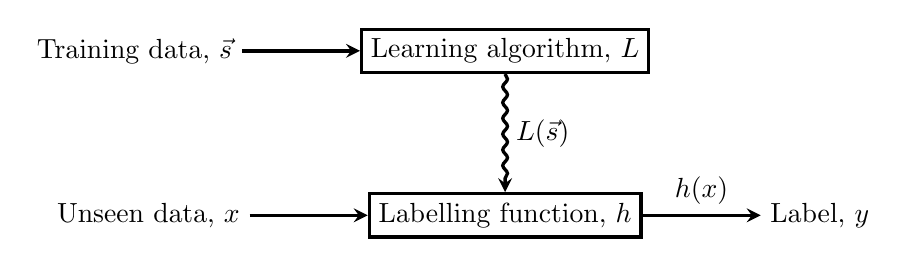
\begin{tikzpicture}[node distance=1.5cm]
	\node[rectangle, very thick, draw] (learning) {Learning algorithm, $L$};
	\node[rectangle, very thick, draw, below = of learning] (inference) {Labelling function, $h$};
	\node[left = of learning] (train) {Training data, $\vec{s}$};
	\node[left = of inference] (uns) {Unseen data, $x$};
	\node[right = of inference] (lab) {Label, $y$};
	
	\draw[-stealth, very thick] (train) -- (learning);
	\draw[-stealth, very thick, decoration={snake, segment length=2mm, amplitude=0.3mm, post length=1.5mm}, decorate] (learning) -- node[right] {$L(\vec{s})$} (inference);
	\draw[-stealth, very thick] (uns) -- (inference);
	\draw[-stealth, very thick] (inference) -- node[above] {$h(x)$} (lab);
\end{tikzpicture}
\end{document}
